\chapter{提案手法の有効性検証}

\section{検証の目的}
 提案手法の有効性を検証するための実験を行った. 本研究は, 知識発現\cite{Nishimura2017}における課題に対して, 指導現場での対話収集とLLMの活用という複合的なアプローチによる解決を提案している. 具体的には, 以下の2点を主な評価項目とした.\\
\begin{enumerate}
    \item 指導現場での知識抽出の有効性:\\
    指導現場おいて, 指導者の発話内容や学習者との対話から, プロセス知識に含まれていない新たな知見が得られるかを検証する. 
    \item LLMによる知識抽出支援の有効性:\\
    収集された指導事例からLLMが提案する改良点が, 実際の指導内容を適切に反映しているか, また体系的な知識整理に寄与しているかを検証する. これは, 記述漏れの検出や知識の体系化という課題に対するLLMの有効性を示すものである. 
\end{enumerate}


\section{実験方法}
\subsection{実験環境}
 本実験は, 石川県内のダンススタジオの協力を得て実施した. 実験協力者として指導者2名と学習者13名が参加した. 指導者の経験年数は, 指導者Aが35年, 指導者Bが30年であった. また, 学習の中で経験年数を回答した8名のうち5名が経験年数1年, 2名が2年, 1名が3年であった.なお, 本実験は本学(北陸先端科学技術大学院大学)の知識科学倫理審査会議の承認(承認コードKSEC 人04-038)に基づいており, 実験協力者に対しては実験の目的, データの収集・利用方法, 個人情報の保護, 参加の任意性等について説明を行い, 同意を得た. \\
 実験対象として社交ダンスのクカラチャを選定した. 社交ダンスを選定した理由は, これまで知識発現が対象としてきた製造業や介護現場とは異なる特徴を持つと考えられるためである. 製造業や介護の現場では, 作業手順や判断基準といった知識を, 実務経験から想起して言語化することが求められる. これに対して社交ダンスでは, 動作の正確さを客観的な基準で判断することが本質的に困難であると考えられる. 例えば「美しい」アームワークや「良い」ステップといった評価は, 指導者の主観的な理解に基づいている. そのため指導者は, 自身が持つ評価基準や動作の意図を, その場で学習者が理解できる形に言語化して伝える必要がある. このとき, 「腕の高さをここまで上げる」「体重移動のタイミングをここで行う」といった具体的な指示から, 「なぜその動きが必要か」「どのような効果を意図しているか」といった原理的な説明まで, 様々な知識が自然と言語される可能性がある. \\
 さらに, この言語化は学習者の実践に基づいて行われる. 例えば製造業では, 作業の結果が製品の品質として客観的に評価できるため, 指導者は事前に想定される状況に対する判断基準を説明することができる. 一方, 社交ダンスでは学習者が実際に動作を行う中で「なぜこの動きがうまくいかないのか」「どうすれば改善できるのか」といった具体的な疑問が生まれ, それに応える形で指導者の持つ知識が表出されると考えられる. これは, ワークショップのように意図的に知識を想起する場合とは異なり, 実践の文脈に即した形で必要な知識が引き出されることを意味する. \\
 また, 社交ダンスの中でもクカラチャを選定した理由は, クカラチャはルンバの基本となるステップであり, 社交ダンスにおいて特に重要な技術だからである. \\
 こうした理由から, 提案手法の有効性検証の題材として社交ダンスのクカラチャを選定した.\\
\\


\subsection{実験手順}
\subsubsection{プロセス知識の構築}
 初めに, 知識発現手法に基づき, クカラチャのプロセス知識を構築した. まず社交ダンスの教科書を基に初期のプロセス知識を作成した. その後, オンライン会議システム(Zoom)を用いて指導者へのヒアリングを実施し, 内容の確認と改良を行った. これを本検証のベースとなるプロセス知識とした.\\


\subsubsection{データ収集の基本手順}
 実験期間は2023年10月16日から11月13日までの約5週間とした. 動作の撮影にはスマートフォンのカメラを使用し, システムへのアクセスについては指導者はPCを, 学習者は各自のスマートフォンを使用した. なお, 学習者の参加回数は個人によって1回から3回まで幅があった. また, クカラチャの実践時に使用した音楽は「Maroon5 Memories」であった.\\
 実験開始時に, 指導者と学習者に対して各種システムの使用方法を説明し, 実際の操作を体験する機会を設けた. 具体的には, アノテーションシステムへのログイン方法, 動画の視聴方法, コメントの確認方法, およびチャット機能の使用方法について説明を行った.\\
 週1回のレッスン日における基本的なデータ収集の手順は以下の通りである.\\
\begin{enumerate}
    \item 指導者がクカラチャの基本動作について説明と実演を行い, 学習者が練習を行った
    \item 研究者が学習者の動作をスマートフォンで撮影し, システムにアップロードした. 撮影の際は, 学習者の全身が画角に収まるよう配慮した
    \item レッスン後, 指導者がPCを使用して動画に指導コメントを付与した
    \item 次のレッスンまでの1週間の間に, 学習者は付与された指導コメントを確認し, 必要に応じて質問や感想を投稿した. また指導者は質問があれば適宜応答した
\end{enumerate}

\subsubsection{プロセス知識の更新プロセス}
 実験開始時に, 指導者には実験期間中にプロセス知識の改良が必要だと感じた場合は随時更新可能である旨を説明した. これは, 指導現場での気づきやLLMによる改良提案を受けて, プロセス知識をより適切なものに改善していくことを意図したものである. プロセス知識の更新は, (1)実験期間中の指導者からの自発的な更新, (2)実験終了後のLLMの妥当性評価を受けての更新, という2つの機会を設けた.\\

\subsubsection{実験中の改善施策}
 実験の進行に伴い, 以下の改善を実施した.\\

\begin{enumerate}
    \item 指導者の見本動画の追加:\\
    より正確な動作イメージを学習者に共有するために, 指導者の見本動画もシステムにアップロードした.
    \item システム利用状況の把握とフォローアップ:\\
    研究者が定期的にシステムの利用状況を確認し, 必要に応じて操作方法の再説明等のフォローアップを実施した. また, LINEを用いて定期的にシステム利用の促進を行った.
    \item システム利用状況の問題切り分け:\\
    システム利用率の低さの原因を特定するため, 学習者には指導コメントを確認した際に必ず「ありがとうございます」などの返信を行うよう指示した. これにより, コメントを確認していない場合と, 確認したが返信していない場合を区別することが可能となった.
\end{enumerate}


\subsection{評価方法}
 実験期間終了後, 提案手法の有効性を検証するため, 以下の4つの観点から評価を実施した. \\
\begin{enumerate}
    \item 指導現場における新しい知識の抽出可能性
    \item LLMが出力した改良提案の適切性
    \item プロセス知識の改良結果
    \item 学習者による提案手法の受容性
\end{enumerate}
 それぞれの評価の目的と具体的な評価方法は以下の通りである.

\subsubsection{指導現場における新しい知識の抽出可能性の評価}
 本評価の目的は, 指導現場が知識抽出の場として有効に機能するかを検証することである. この評価目的に対し, 収集した指導事例について, 定量的評価と定性的評価を実施した. 定量的評価では, 指導コメント数ややり取り数などの基本統計, およびプロセス知識に含まれない要素(未含有要素)の割合を分析した. 定性的評価では, 指導コメントの内容分類とやり取りの特徴分析を行った.\\
 なお, 未含有要素の判定は研究者(社交ダンス未経験者)が行った. 以下のいずれかに該当する指導コメントを「未含有要素を含む」と判定した.\\
\begin{itemize}
    \item 構造化知識を参照しても理解できない要素を含むコメント
    \item コメントの意図は理解できるが, その内容が構造化知識に明示的に含まれていないコメント
\end{itemize}

\subsubsection{LLMが出力した改良提案の適切性評価}
 本評価の目的は, LLMが知識抽出支援ツールとして有効に機能するかを検証することである. この目的に対し, 定量的評価と定性的評価を実施した. 定量的評価では, 以下の3つの観点から評価を行った.\\
\begin{enumerate}
\item LLMが指導現場から得られた指導コメントとやりとりから未含有要素を抽出できているか
\item LLMが指導現場から得られた指導コメントとやりとりからプロセス知識に既に含まれる要素を除外できているか
\item 改良提案の内容および提案位置が適切かどうか
\end{enumerate}
 このうち, 1と2については先述した研究者による未含有要素, 既存要素の分類を正解データとして, Accuracy, Precision, Recall, F値を評価指標を用いた. 3については出力をしづオシャに評価してもらい, Accuracyを算出した.
また, LLMの出力を得る際は, 入力として全ての指導コメントとやりとりを一度にプロセス知識に紐づけることも技術的には可能だが, 改良提案の適切性をより厳密に評価するため, 本実験では個別に紐づけて評価を行った. \\

\subsubsection{プロセス知識の改良結果の評価}
 本評価の目的は, 提案手法が熟練技能者の持つ知識を実践の中で自然に抽出・整理可能な仕組みとして機能するかを検証することである. この目的に対し, 以下の2つの機会におけるプロセス知識の改良内容を確認した.\\
\begin{enumerate}
\item 実験期間中の自発的な改良:指導者には実験期間中, 気づきがあれば随時プロセス知識を更新可能である旨を伝え, その結果としての改良内容
\item LLMの改良提案を受けての改良:実験終了後, LLMが出力した改良提案の適切性評価を踏まえて実施された改良内容
\end{enumerate}

\subsubsection{学習者による提案手法の受容性評価}
 本評価の目的は, 提案手法が自然な文脈での知識抽出・整理の仕組みとして成立するために必要な, 学習者からの支持が得られているかを検証することである. 指導現場における知識抽出・整理は, 学習者がその仕組みを受け入れ, 積極的に活用することで初めて実現されるためである. この検証のため, 学習者へのアンケート調査(13名中8名が回答)およびシステムの使用感や改善点に関するヒアリングを実施した. アンケートでは以下の項目について調査を行った:\\
\begin{enumerate}
\item 学習者の基本情報
    \begin{itemize}
        \item 社交ダンスを始めた目的
        \item 経験年数
        \item 普段の練習時間・場所
    \end{itemize}
\item 普段の学習方法
    \begin{itemize}
        \item 指導内容の理解・記憶方法
    \end{itemize}
\item システムの利用状況
    \begin{itemize}
        \item システムの確認頻度
        \item システムの利用方法
        \item クカラチャへの理解深化要因
    \end{itemize}
\item 自由記述
    \begin{itemize}
        \item システムの使用感
        \item 本研究への要望
        \item その他感想
    \end{itemize}
\end{enumerate}


\section{評価結果}
 ここでは, 収集したデータに基づいて提案手法の有効性に関する評価結果を示す. まず事前に準備したプロセス知識の概要を説明する. 続いて各評価項目について, 定量的な評価と定性的な評価の結果を示し, これらを踏まえて提案手法の有効性を考察する.




\subsection{事前準備したプロセス知識の概要}
 実験に先立ち, クカラチャの動作を構造化したプロセス知識を作成した. 図\ref{fig:process_knowledge_base}は, その一部であるレフトフットクカラチャ(男子)の動作を示したものである. なお, ライトフットや女子の動作については, 基本的な構造は同じで動作の向きが逆になるのみである.\\

\begin{figure}[htbp]
    \centering
    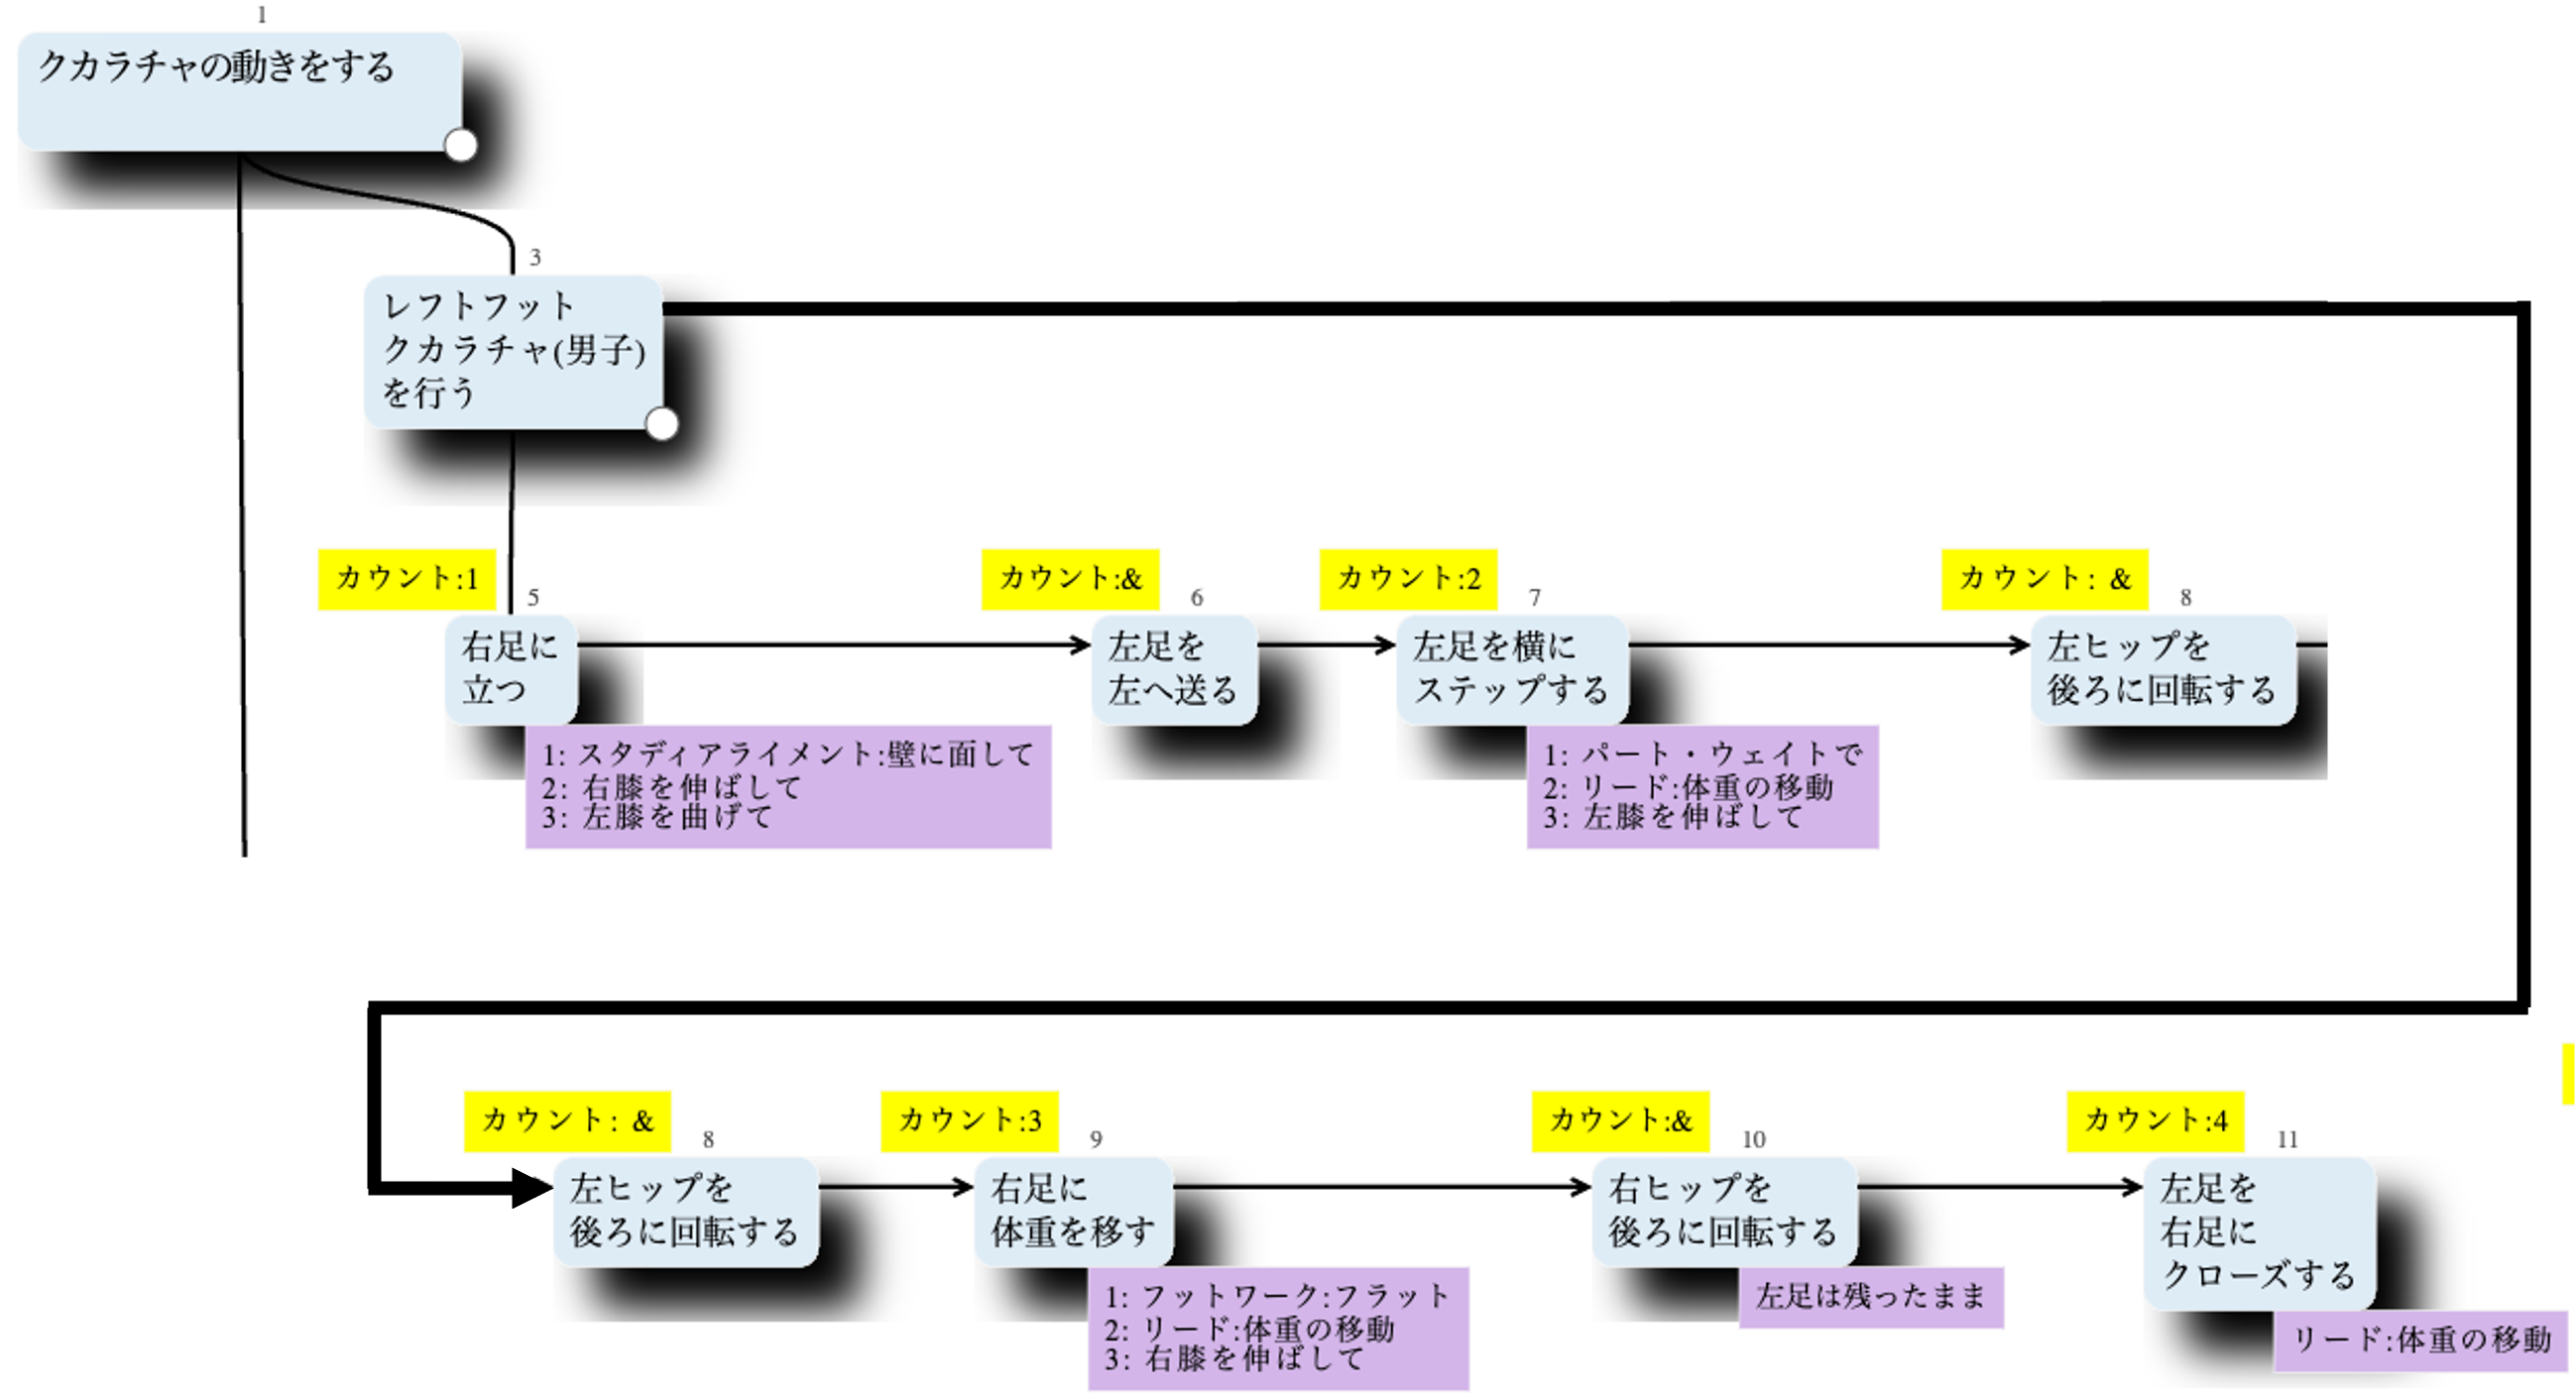
\includegraphics[width=1.0\linewidth]{./image/process_knowledge_base.png}
    \caption{レフトフットクカラチャ(男子)のプロセス知識}
    \label{fig:process_knowledge_base}
\end{figure}

 このプロセス知識は, 7つの基本動作(右足に立つ, 左足を左へ送る, 左足を横にステップする, 左ヒップを後ろに回転する, 右足に体重を移す, 右ヒップを後ろに回転する, 左足を右足にクローズする)で構成されている. それぞれの動作には実行タイミング(カウント)が設定されており, また「スタディアライメント:壁に面して」「パート・ウェイトで」「フットワーク:フラット」といった動作の詳細な指示が付与されている.\\



\subsection{指導現場における新しい知識の抽出可能性の評価}
\subsubsection{定量的評価}
 収集した指導コメントについて, プロセス知識に含まれている要素のみで構成されるもの(以下, 既存要素のみ)と, プロセス知識に含まれていない要素を含むもの(以下, 未含有要素を含む)に分類して分析を行った.\\
 プロセス知識との対応関係について, 既存要素のみで構成されるものが12件(約24\%), 未含有要素を含むものが37件(約76\%)であった. この37件の未含有要素を含むコメントのうち, 指導者1のコメントが12件, 指導者2のコメントが25件を占めていた.\\
 やり取りの特徴として, 全49件の指導コメントのうち18件(約37\%)に学習者とのやり取りが存在した. やり取りの回数については, 1回のやり取りで終了したものが16件, 3回のやり取りに及んだものが2件であり, 1つの指導コメントに対する平均やり取り数は1.22回であった.\\

\subsubsection{定性的評価}
 収集された指導コメントには, プロセス知識を詳細化する指導と, プロセス知識に記載のない新しい部位に関する指導が見られた.\\
 プロセス知識を詳細化する指導では, 「踏み替えのタイミングが早い」「左足に体重が乗る前にヒップが回転してしまっている」といった動作の順序やタイミングに関する指摘や, 「軸が左足内側まで乗るように」「踏みかえの体重移動をはっきりと」といった体重移動の詳細な方法に関する指導が含まれていた. また,「ヒップと一緒にももも外側に回転させる」「左のヒップを回転した時に左の内ももを後ろにひく」といった既存の動作要素をより詳細に説明する指導や, 「ボディの移動は早く, ヒップのアクションはゆっくり見せるとメリハリがでる」といった動作の質に関する指導も見られた.\\
 プロセス知識に記載のない新しい部位に関する指導としては, 「ボディをストレッチ」「上半身, アームの動きがぎこちない」「上半身が揺れて傾いてしまう」といった上半身の使い方に関する指導が見られた. これらはプロセス知識では言及されていなかった身体部位の動きについて説明するものであった.\\
 やり取りについては, 全22件中16件が「ありがとうございます」といった単純な確認や感謝のコメントであった. 一方で, 残りの6件では指導内容に関する具体的なやり取りが見られた. 例えば, 「体重移動しながら回転させてしまってる」という学習者の質問に対し, 指導者が「歩幅を少し狭めた方が体重移動とヒップの回転を分けられる」と回答するなど, 対話を通じてプロセス知識には含まれていない動作の詳細が明らかになる場面も観察された.\\

\subsubsection{知識抽出の場としての有効性}
 定量的な評価と定性的な評価の結果から, 指導現場が知識抽出の場として効果的に機能することが確認された. まず, 収集された指導コメントの76\%(37件)に未含有要素が含まれていたことは, 指導現場が新たな知識を抽出する機会を多く含んでいることを示している.\\
 定性的評価で示したように, 指導現場では2つの方向で知識が抽出されていた. 1つ目はプロセス知識の詳細化である. 体重移動の詳細な方法や動作の質的な側面など, プロセス知識では表現しきれていなかった要素が具体的な指導を通じて明らかになった. 特に動作の順序やタイミングに関する指摘は, プロセス知識で示された基本的な動作の関係性をより正確に理解する上で重要な知見となった.\\
 2つ目は上半身の使い方など, プロセス知識では言及されていなかった新しい部位に関する指導である. これらの指摘は, クカラチャの動作がプロセス知識に記述された下半身の動きだけでなく, 全身の協調的な動きとして捉える必要があることを示している.\\
 さらに, 37\%の指導コメントで学習者とのやり取りが確認された. その中でも特に注目すべきは, 学習者からの具体的な質問に対する指導者の回答を通じて新たな知識が表出される場面である. 定性的評価で示した体重移動と回転の分離に関するやり取りは, 学習者の問題提起が新たな指導内容を引き出すきっかけとなることを示す例である.\\
 このように, 指導現場では, プロセス知識の詳細化や新たな知識要素の発見が自然な形で行われることが確認された. 特に学習者との対話は, プロセス知識には含まれていない要素を引き出す重要な機会となっていた.\\
 一方で, やり取りの発生は全指導コメントの37\%にとどまり, そのうち73\%(16件)は「ありがとうございます」といった確認や感謝のコメントであった. このことは, 指導現場での双方向のコミュニケーションを十分に引き出せていない可能性を示している. この要因については, 後述する学習者へのアンケート結果から示唆が得られている.\\
 これらの結果は, 指導現場が知識抽出の場として大きな可能性を持つことを示している. 特に, プロセス知識の詳細化と新たな知識要素の発見という2つの方向性での知識抽出が確認されたことは, 提案手法の有効性を支持するものである. しかしながら, 双方向コミュニケーションの活性化という点では課題が残されており, より効果的な知識抽出を実現するためには, 学習者の積極的な参加を促す仕組みの改善が必要であることも明らかになった. 


\subsection{LLMが出力した改良提案の適切性評価}
\subsubsection{定量的評価}
 LLMが分析した改良点と提案内容について, 未含有要素の抽出と既存要素の除外, および改良提案の適切性という3つの観点から評価を行った.\\
 まず, プロセス知識との対応関係に着目した評価結果を表\ref{table_llm_extraction}に示す.

\begin{table}[htbp]
    \centering
    \begin{tabular}{l|rrrr}
        \hline
        評価項目 & Accuracy & Precision & Recall & F値 \\ \hline
        未含有要素の抽出 & 0.865 & 0.941 & 0.914 & 0.928 \\
        既存要素の除外 & 0.583 & 0.500 & 0.200 & 0.286\\
        \hline
    \end{tabular}
    \caption{LLMによる要素の抽出・除外の評価結果}
    \label{table_llm_extraction}
\end{table}

次に, LLMによる改良提案の評価結果を表\ref{table_llm_proposal}に示す. ここでは, 指導現場で収集した指導コメントやそのやり取りから直接的に導かれる「指導事例に基づく提案」と, LLMが持つ知識に基づいて補完的に生成する「指導事例に基づかない提案」に分けて評価を行った.

\begin{table}[htbp]
    \centering
    \begin{tabular}{l|l|rrrr}
        \hline
        提案の種類 & 評価観点 & Accuracy \\ \hline
        \multirow{2}{*}{指導事例に基づく提案} & 内容 & 0.780 \\
        & 位置 & 0.361 \\ \hline
        \multirow{2}{*}{指導事例に基づかない提案} & 内容 & 0.254 \\
        & 位置 & 0.182 \\
        \hline
    \end{tabular}
    \caption{LLMによる改良提案の評価結果}
    \label{table_llm_proposal}
\end{table}

 評価結果から, LLMは新規要素の抽出に高い精度を示し(Accuracy: 0.865), 指導事例に基づく改良提案については内容面での適切性が高いことが確認された(Accuracy: 0.780). 一方で, 既存要素を適切に除外すること(Accuracy: 0.583)や, 改良提案の位置の特定(指導事例に基づく提案でAccuracy: 0.361, 指導事例に基づかない提案でAccuracy: 0.182)については大きな課題が残ることが明らかになった. さらに, 指導事例に基づかない独自の提案についても, 内容面での適切性が低い(Accuracy: 0.254)という結果となった.

\subsubsection{定性的評価}
 LLMが出力した改良提案について, 指導者へのヒアリングから, 以下のような特徴が明らかになった. \\
 収集した指導コメントの中には, LLMが適切な改良提案を行えたものがあった. 例えば「もう少しボディーをストレッチ」といった指導コメントに対して, LLMは「左足を横にステップする」と「左ヒップを後ろに回転する」の間に「上半身のストレッチを行う」という新しい行為ノードを追加し, その具体的な実現方法として「ボディとヒップにずれを作る」「左側に上半身を伸ばす」という動詞の詳細を追加する提案を行った. このように具体的な動作の質を向上させる提案は, プロセス知識の改良においても指導者が参照するなど, 高く評価された. \\
 しかし多くの改良提案において, 指導コメントを単に言い換えたり抽象化したりする傾向が見られた. 例えば「踏みかえの体重移動をはっきりと」「つま先を外側に向けて」といった指導コメントをそのまま動詞の詳細として追加する提案や, 「ヒップと一緒にももも外側に回転させる」という指導コメントに対して「ももを外側に意識する」といった抽象的な表現に置き換えるだけの提案が多く見られた. \\
 指導者へのヒアリングを通じて, クカラチャの動作には4つのコアとなる要素があることが明らかになった. これらは, 指導者がLLMの改良提案に対して行ったフィードバックを分析することで特定された. 第一に「つま先を外側に向ける」という要素は, 例えば「左右のかかとが離れないようにつけて踏みかえ」「クローズする足のつま先が内側に向かないようによせる」といった一見異なる指導コメントに対して, 指導者が「つま先を外に向けるという意図」というフィードバックを残していたことから確認された. 第二に「軸を床に対して垂直に保つ」という要素は, 「アームの収まりが弱い」「体重移動は左足内側まで背骨を移動させる」などの指導コメントに対して「軸をまっすぐにするための指導」「体の軸をまっすぐにして欲しかったという意図」というフィードバックが得られたことから特定された. 第三の「脚をだす, 体重を移動する, ヒップを回転するを分ける」という要素は, 「ヒップの回転が早い」「下半身のアクションがすべて一緒になっている」という指導コメントに対して「これら3つの動作を分けることが重要」「ここでは動作を区切ることを教えている」というフィードバックから導かれた. 第四の「常に床に力をかけ続ける」という要素は, 「ヒップを後ろに回転させたらヒールをしっかり床につく」「ヒップを回転させているときに右のひざが曲がらないようにする」といった指導コメントに対する「床にプレッシャーをかけ続けるという意図」「膝を曲げないのは床に力をかけ続けるため」というフィードバックから確認された. \\
 これらの4つの要素に対するLLMの改良提案を具体的に見ると, 「ヒップの回転が早い」という指導コメントについて, 「左足を横にステップする」という行為ノードの動詞の詳細として「ヒップの回転を抑制する」「上半身の姿勢を維持する」といった要素を追加することを提案していた. また, 「もう少し体重をのせてからヒップを回転」という指導コメントに関しては, 「背骨と骨盤の位置を保つ」という新しい行為ノードを追加し, その動詞の詳細として「背骨と骨盤が真っ直ぐに保たれているように意識する」といった姿勢に関する要素を提案していた. さらに「体重移動をする時に軸足にしっかりのっていることを意識する」という指導コメントについては, 「体重移動を意識する」という行為ノードを追加し, プロセス知識の改良を試みていた. これらの提案に対して指導者から「指導コメントをそのまま追加しているだけ」といったフィードバックが多く見られたことから, LLMは個々の指導コメントの背後にある本質的な要素を読み取ることができていないことが確認された. \\

\subsubsection{知識抽出支援ツールとしての適切性}
 定量的評価と定性的評価の結果から, LLMの知識抽出支援ツールとしての特性について考察する. \\
 まず, LLMは指導コメントから未含有要素を抽出する基本的な能力を有していることが確認された. 未含有要素の抽出におけるF値が0.928という結果は, LLMが高い精度で新規の知識要素を特定できることを示している. 「もう少しボディーをストレッチ」といった指導コメントから具体的な動作の質を向上させる提案ができた事例も確認された. \\
 しかし, 多くの改良提案において指導コメントの表層的な言い換えや抽象化に留まっており, 指導の背景にある本質的な意図を捉えることができていなかった. 特に, 指導者へのヒアリングから明らかになった4つのコアとなる技術要素(「つま先を外側に向ける」「軸を床に対して垂直に保つ」「脚をだす, 体重を移動する, ヒップを回転するを分ける」「常に床に力をかけ続ける」)は, 様々な表現で指導されていたにもかかわらず, LLMはそれらの指導コメントの背後にある共通の技術的要素を読み取ることができなかった. \\
 このことから, 現状のLLMは表面的な未含有要素の抽出には有用であるものの, 指導の背景にある本質的な技術要素を抽出するという観点では, 単独での活用には限界があることが示唆された. 今回の実験条件では, LLMに指導者の技術的知識や意図に関する事前情報が与えられていなかったことも, この限界の一因として考えられる. \\
 これらの結果は, 提案手法においてLLMは未含有要素の特定という基礎的な支援ツールとしては機能するものの, より深い技術的理解を要する知識抽出には人間の専門的な解釈が必要不可欠であることを示している. \\


\subsection{プロセス知識の改良結果の確認}
実験を通じて, プロセス知識は2回の機会で改良された. それぞれの機会において, 指導者1と指導者2の両名に改良の機会が与えられた. 1回目は実験期間中の自発的な改良機会であり, 2回目は実験終了後にLLMの改良提案を評価した上での改良機会である. \\

\subsubsection{実験期間中の自発的な改良}
 実験期間中の指導者1による改良では, 動作の質に関する詳細な説明が追加された(図\ref{fig:process_knowledge_instructor1_ver1}). 具体的には, 上半身の使い方に関する指示(「左アームを開き始める(肘を外側に向ける)」「左アームを横に開く」など)が各動作に追加され, また体重移動に関する具体的な指示(「ボディとヒップが足の上まで」)や, 歩幅や膝の使い方に関する注意点(「歩幅が広くならないように(肩幅程度)」「右膝が緩まないように」)など, より詳細な動作の質に関する説明が加えられた. さらに, 「つま先を外側に向けて」という常時の注意事項が新たに追加された. 一方, 動作の基本的な順序(右足に立つ→左足を左へ送る→左足を横にステップする→左ヒップを後ろに回転する→右足に体重を移す→右ヒップを後ろに回転する→左足を右足にクローズする)は維持された. 

\begin{figure}[htbp]
    \centering
    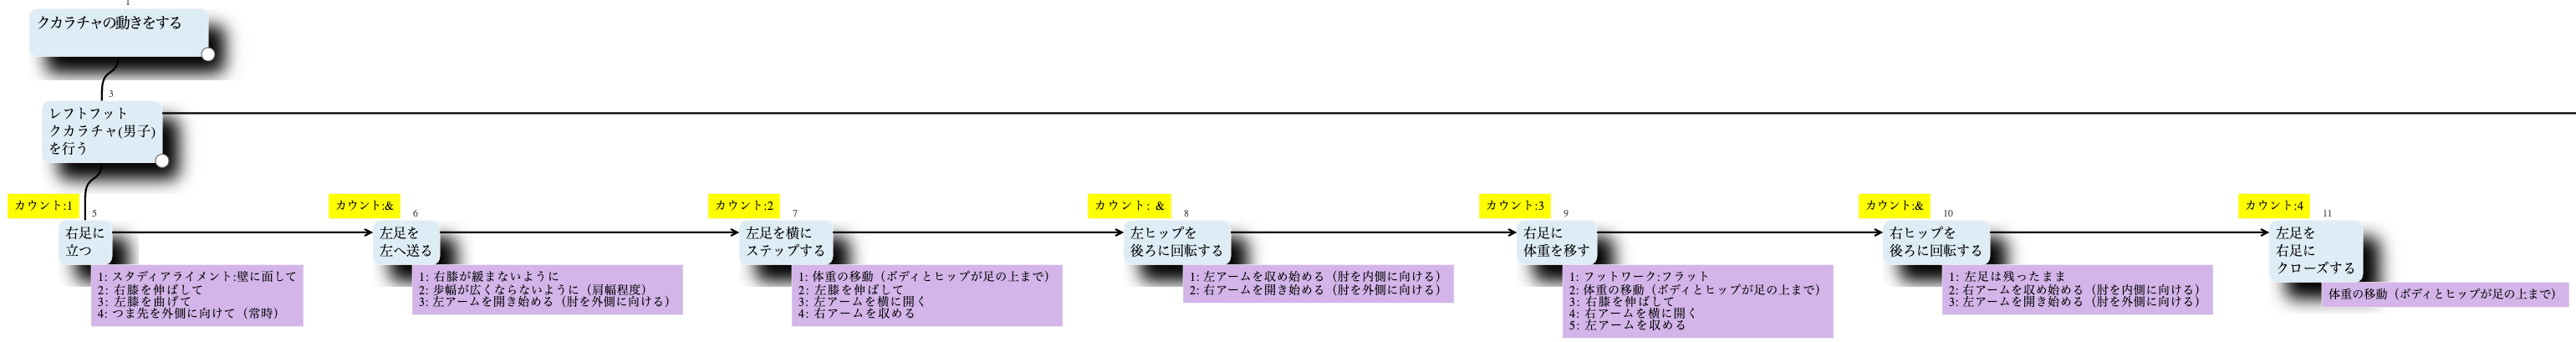
\includegraphics[width=1.0\linewidth]{./image/process_knowledge_instructor1_ver1.png}
    \caption{実験期間中に指導者1によって改良されたプロセス知識}
    \label{fig:process_knowledge_instructor1_ver1}
\end{figure}

指導者2は, この段階では改良を行わなかった. 

\subsubsection{LLMの改良提案を受けての改良}
 次に, 実験終了後にLLMの改良提案を評価した上で, 指導者1がさらなる改良を行った(図\ref{fig:process_knowledge_instructor1_ver2}). この改良では, 上半身の使い方に関するより具体的な指示が追加された. 特に「左足を横にステップする」動作において, 「上半身のストレッチを行う」「ボディとヒップにずれを作る」「左側に上半身を伸ばす」という詳細な指示が加えられた. これはLLMが抽出した「ボディーをストレッチ」という指導コメントに対応する改良であり, 上半身の使い方をより具体的に示すものとなっている. \\

\begin{figure}[htbp]
    \centering
    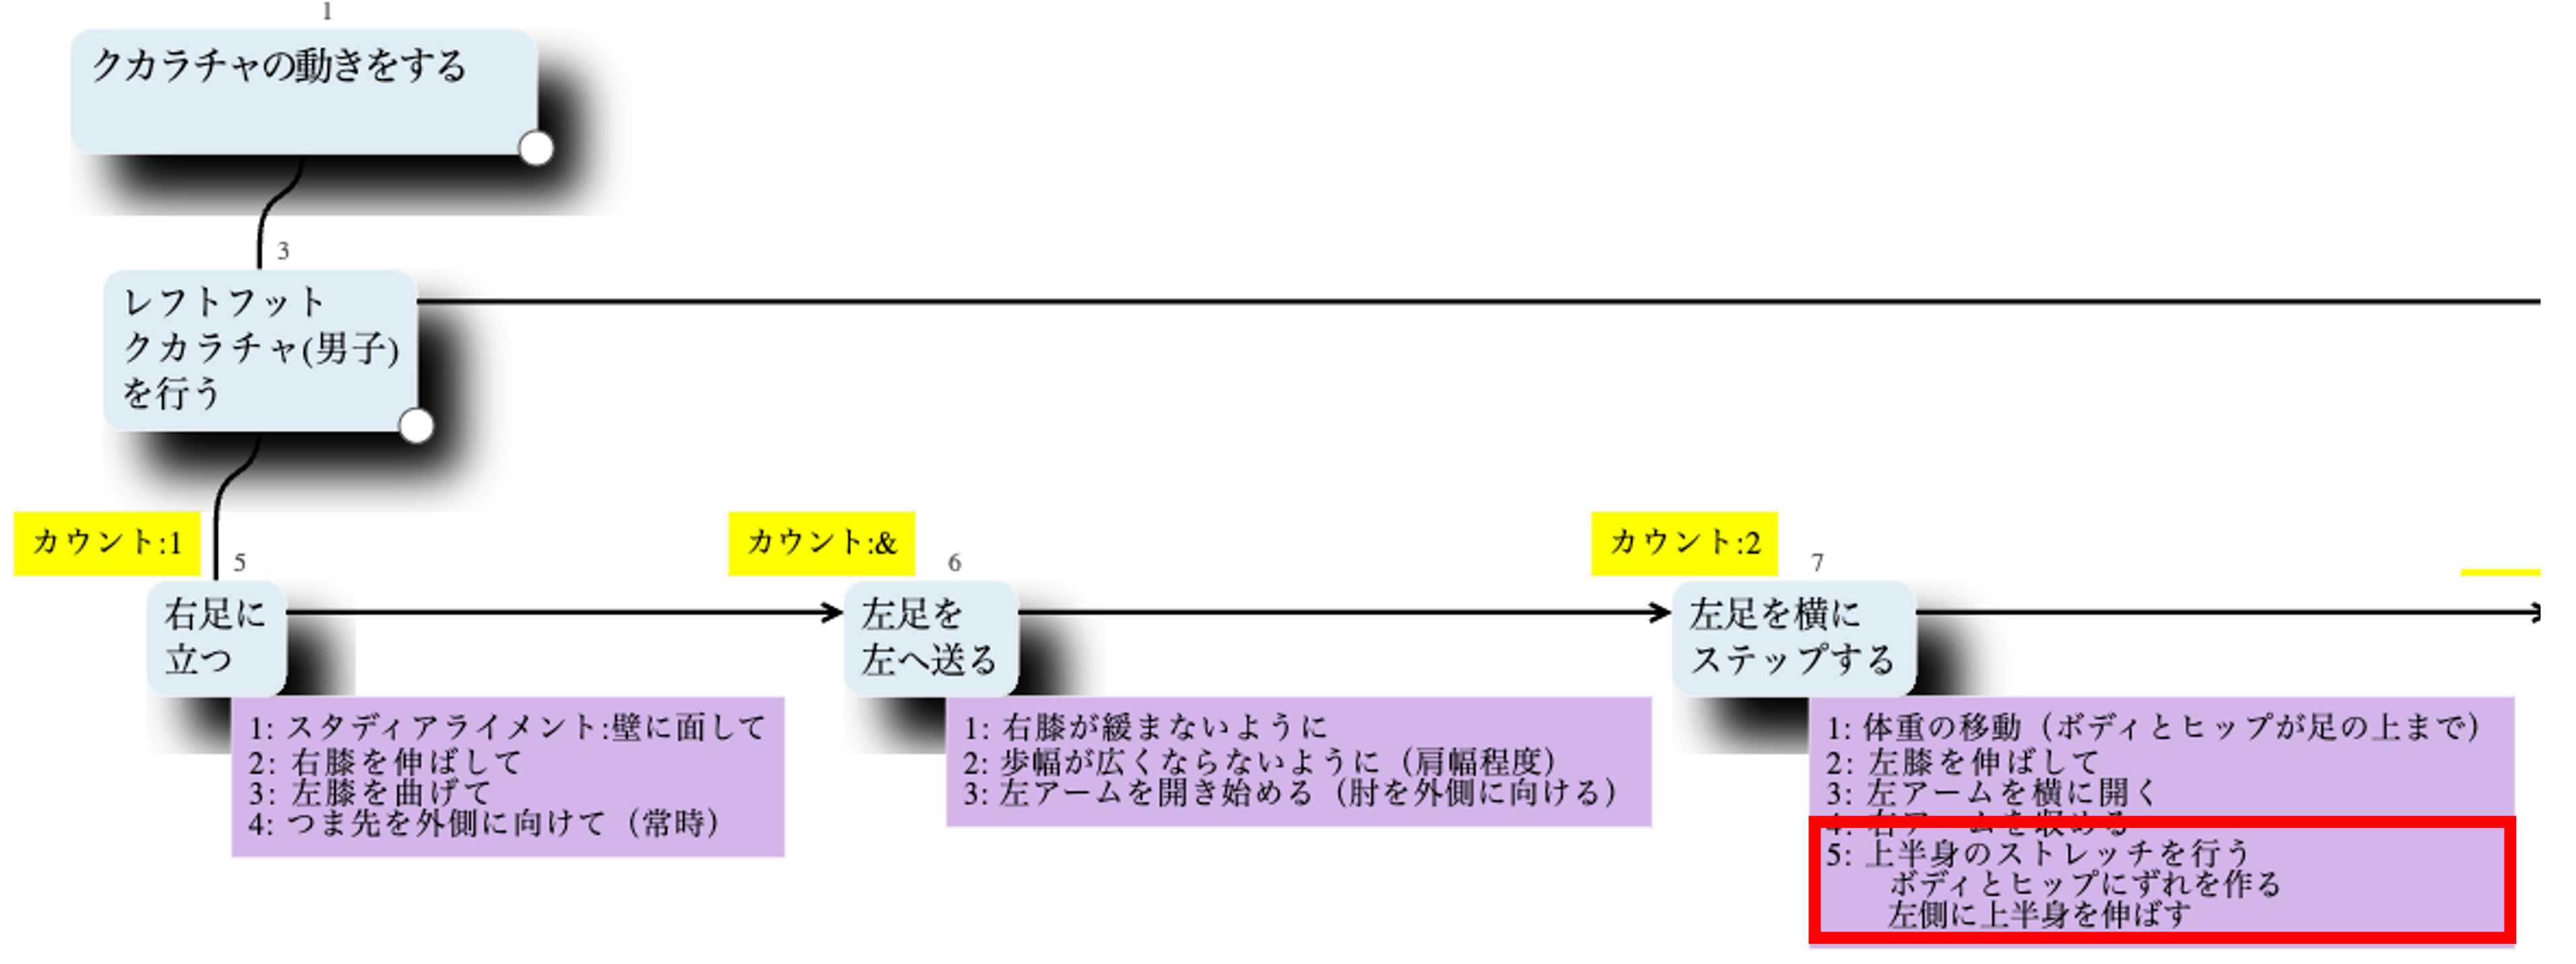
\includegraphics[width=1.0\linewidth]{./image/process_knowledge_instructor1_ver2.png}
    \caption{LLMのフィードバック後に指導者1によって改良されたプロセス知識}
    \label{fig:process_knowledge_instructor1_ver2}
\end{figure}

 一方, 指導者2は特に2つの重要な要素を追加する改良を行った(図\ref{fig:process_knowledge_instructor2_ver1}). 第一に, 「つま先は外側に向ける(継続)」という注意点が動詞の詳細として追加された. これは各動作において常時意識すべき基本的な姿勢要素として位置づけられている. 第二に, 「軸に関して:背骨が上から吊り下がっている感じ, 頭と背骨が床に対して垂直になるイメージ」という軸の保持に関する具体的な説明が追加された. これは抽象的な「軸を保つ」という指示を, より具体的なイメージとして学習者に伝えるものとなっている. \\
 これらの改良の特徴として, 実行タイミング(カウント)や基本的な実行方法(パート・ウェイト, フットワーク等)といった基本的な要素は変更されていない点が挙げられる. 追加された要素は, 動作全体を通じて意識すべき基本的な姿勢や動きの質に関するものであり, 個々の動作の変更ではなく, 動作全体の質を向上させるための指示となっている. これらの改良によって, プロセス知識はより実践的で具体的なものとなり, 学習者がより正確に動作をイメージし, 実行できるようになることが期待される. \\

\begin{figure}[htbp]
    \centering
    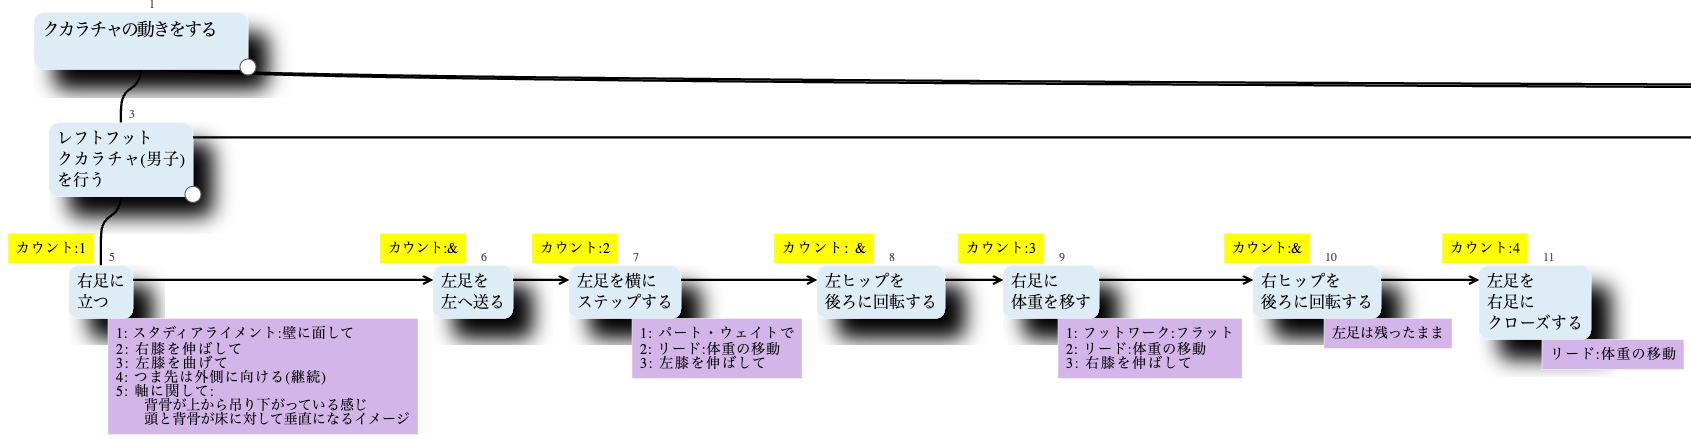
\includegraphics[width=1.0\linewidth]{./image/process_knowledge_instructor2_ver1.png}
    \caption{LLMのフィードバック後に指導者2によって改良されたプロセス知識}
    \label{fig:process_knowledge_instructor2_ver1}
\end{figure}

\subsubsection{提案手法の実現可能性に関する評価}
 プロセス知識の改良結果から, 提案手法が知識抽出・整理の仕組みとして機能することが確認された. これは以下の2つの観点から評価できる.  \\

 第一に, 指導現場での知識抽出が限定的ながら実現されている. 実験期間中, 指導者1は上半身の使い方や体重移動, 歩幅や膝の使い方など, より詳細な動作の質に関する説明を自発的に追加した. これは, 指導活動の中で新たな知識要素を抽出し, それをプロセス知識として形式化できる可能性を示している.  \\

 第二に, LLMの改良提案を介した知識の追加が確認された. 実験終了後, 両指導者はLLMの改良提案を評価した上で, それぞれ異なる観点からプロセス知識を改良している. 指導者1は上半身の使い方に関するより具体的な指示を追加し, 指導者2は姿勢の基本要素に関する詳細な説明を加えた. このことは, LLMを介することで, プロセス知識の改良機会を創出できる可能性を示している.  \\

 一方で持続可能性という観点からは課題が残る結果となった. 実験期間中の自発的な改良は指導者1のみにとどまり, 指導者2は実験終了後のLLMの改良提案を受けてはじめて改良を行った. また, プロセス知識の改良は2回の機会に限定されており, 継続的な改良のサイクルは確認できなかった. このことは, 指導現場での自然な文脈の中で知識抽出・整理の仕組みとして定着させるためには, 自発的な知識抽出を促す仕組みや, より頻繁な改良機会の設定など, さらなる改善が必要であることを示している.  \\

 これらの結果から, 提案手法は指導現場での知識抽出とLLMを活用した知識の追加という2つのアプローチを組み合わせることで, 基本的な知識抽出・整理の仕組みとして機能し得ることが示された. ただし, 持続可能な仕組みとして確立するためには, 特に指導現場での自発的な知識抽出を促進するための改善と, より継続的な改良サイクルを実現するための工夫が必要であると考えられる.  \\

\subsection{学習者による提案手法の受容性評価}
 提案手法が学習者にとって受け入れられ, 効果的な学習支援となり得るかを評価するため, 実験参加者13名中8名(約62\%)からアンケート回答を得た. \\
 回答者の背景として, 全員が週1回以上ダンススタジオで練習を行っていた. 普段の指導内容の理解方法としては, 全員が「積極的に体を動かしながら感覚的に理解する」を選択しており, その他「頭の中で整理しながら理屈で理解する」「レッスン時に先生に質問する」などの方法を組み合わせていた. \\
 システムの利用状況については, 大半の学習者が「レッスン時のみ」の利用にとどまっていた. 利用が限定的だった理由として, 「レッスン時間外にダンスについて考える機会が少なかった」「日常生活が忙しく確認する時間がなかった」「スマートフォンでの操作が面倒だった」などが挙げられた. 一方で, 「先生のコメントを確認するために利用した」「自分の動作や先生のお手本の確認のために利用した」という積極的な利用も一部で見られた. \\
 クカラチャへの理解深化要因については, 「先生からのコメントで理解を深めることができた」という回答が最も多く, 次いで「構造化知識を見ることで理解を深めることができた」「先生の見本動画を見ることで理解を深めることができた」といった回答が得られた. これは提案手法の各要素が学習者の理解促進に一定の効果を持つことを示唆している. \\
 システムに対する要望として, 「大きな画面でもコメントが確認できると良い」「スマートフォンの画面の比率に対応していると学習者が利用しやすい」「コメントが入った時の通知機能があれば良い」といった操作性に関する改善点が指摘された. また「参考資料が比較的少ない」という意見も見られた. 
 これらの結果から, 提案手法は学習者の理解促進に一定の効果を持つことが示された一方で, 日常的な利用を促進するためには, 操作性の改善や通知機能の追加など, より使いやすいインターフェースの実現が必要であることが明らかになった. \\


\section{提案手法の総合的な評価}
 これらの評価結果から, 本研究の目的に対する達成度を以下のように評価することができる. \\
 第一に, 指導現場での知識抽出については, 指導者と学習者の自然な対話から新たな知識要素を抽出することに成功し, その有効性が確認された. 特に, 指導者のコメントの76\%に未含有要素が含まれていたことは, 普段の指導活動の中で知識抽出が可能であることを示している. \\
 第二に, LLMによる知識抽出支援については, 未含有要素の抽出において高い精度(F値0.928)を示し, 知識の体系的な整理に貢献できることが確認された. しかし同時に, 指導の本質的な意図の理解には課題が残ることも明らかになった. \\
 これらの結果は, 本研究が目指したより自然な文脈での知識抽出・整理の仕組みの実現に向けて, 基本的な枠組みは確立できたものの, さらなる改善の余地があることを示している.\\